%
% $RCSfile: database_server.tex,v $
%
% Copyright (C) 2002-2008. Christian Heller.
%
% Permission is granted to copy, distribute and/or modify this document
% under the terms of the GNU Free Documentation License, Version 1.1 or
% any later version published by the Free Software Foundation; with no
% Invariant Sections, with no Front-Cover Texts and with no Back-Cover
% Texts. A copy of the license is included in the section entitled
% "GNU Free Documentation License".
%
% http://www.cybop.net
% - Cybernetics Oriented Programming -
%
% http://www.resmedicinae.org
% - Information in Medicine -
%
% Version: $Revision: 1.1 $ $Date: 2008-08-19 20:41:06 $ $Author: christian $
% Authors: Christian Heller <christian.heller@tuxtax.de>
%

\section{Database Server}
\label{database_server_heading}
\index{Database Server}
\index{Database Management System}
\index{DBMS}
\index{Database}
\index{DB}
\index{2 Tiers}
\index{Persistent Data}
\index{Transient Data}
\index{Querying}
\index{Transaction Handling}
\index{Locking}
\index{Hierarchical DBMS}
\index{Network DBMS}
\index{Relational DBMS}
\index{RDBMS}
\index{Object-Relational DBMS}
\index{ORDBMS}
\index{Object-Oriented DBMS}
\index{OODBMS}
\index{Data Definition Language}
\index{DDL}
\index{Structured Query Language}
\index{SQL}
\index{Object-Relational DBMS}
\index{Object-Oriented Model}
\index{OOM}
\index{Entity-Relationship Model}
\index{ERM}
\index{Object Query Language}
\index{OQL}
\index{Middleware}
\index{Java Database Connectivity}
\index{JDBC}
\index{Open Database Connectivity}
\index{ODBC}
\index{Enterprise Java Beans}
\index{EJB}
\index{Business Objects}
\index{BO}

Another popular kind of server system, besides the application server, is the
\emph{Database Server}, also called \emph{Database Management System} (DBMS).
It manages structured data called a \emph{Database} (DB) and serves clients
with \emph{persistent} data. The arrow in figure \ref{database_figure} points
in the direction into which the application server sends its queries to the
database server, in order to retrieve data. Example DBMS representatives are
\emph{PostgreSQL}, \emph{MySQL}, \emph{DB2}, \emph{ORACLE}, \emph{ObjectStore},
\emph{POET} or \emph{Versant}.

\begin{figure}[ht]
    \begin{center}
        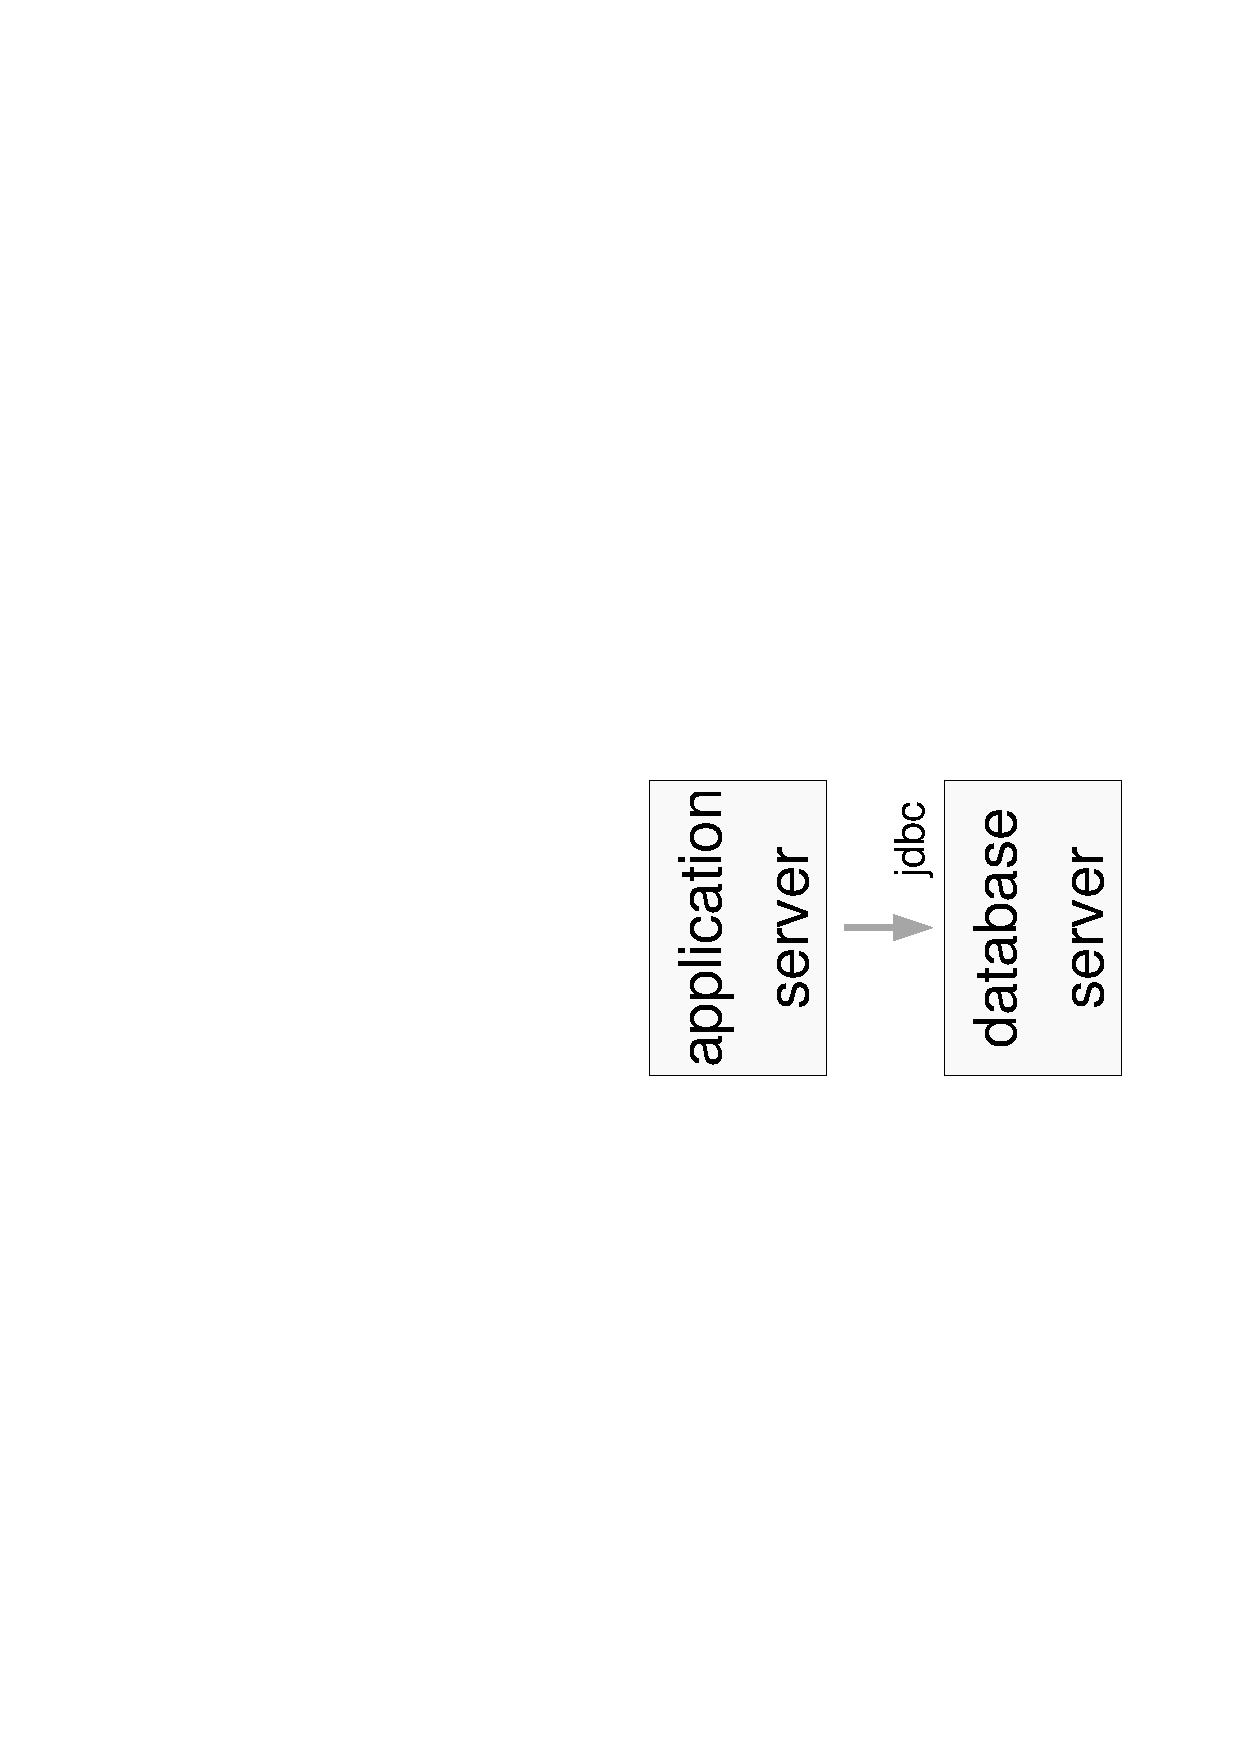
\includegraphics[scale=0.3,angle=-90]{graphic/database.pdf}
        \caption{Database Server (2 Tiers)}
        \label{database_figure}
    \end{center}
\end{figure}

\emph{Persistent Data} are those that live longer than the system working on them.
Very often, this is domain-specific- but also configuration information. These
are stored in a filesystem or database \cite{zimmermann}. \emph{Transient Data},
on the other hand, is temporary information that a system holds during its
lifetime, to function correctly. They get destroyed together with the system
which created them.

Managing persistent data implies a number of quite complex tasks, the details of
which will not be part of this document. To these aspects of database servers
belong:

\begin{itemize}
    \item[-] Querying
    \item[-] Transaction Handling
    \item[-] Locking
\end{itemize}

Different types of database systems exist. The major ones are:

\begin{itemize}
    \item[-] \emph{Hierarchical and Network DBMS}
    \item[-] \emph{Relational DBMS} (RDBMS)
    \item[-] \emph{Object-Relational DBMS} (ORDBMS)
    \item[-] \emph{Object-Oriented DBMS} (OODBMS)
\end{itemize}

Hierarchical DBMS were the first (electronic) databases ever used. They managed
their data in tree structures, starting each access from the root node. Network
DBMS went one step further: data could be associated at will \cite[p. 128]{zimmermann}.
Relational DBMS are based on tabular data structures which can have relations.
They were the first to accomplish a true separation between application and data.
Special languages were created to define and query such data sources: The
\emph{Data Definition Language} (DDL) and the \emph{Structured Query Language}
(SQL). Object-Relational DBMS were to fill the semantic gap between
\emph{Object-Oriented Model} (OOM) and \emph{Entity-Relationship Model} (ERM)
structures. Their extensions introduced a number of user-defined data types.
Object-Oriented DBMS conclusively close the semantic gap between object-oriented
applications and data. Their programming interface is often integrated into a
framework. The new SQL-based \emph{Object Query Language} (OQL)
\cite[p. 138]{zimmermann} was created for them.

The communication between systems can be eased with special techniques. After
Tanenbaum \cite{tanenbaum2002}, these were often called \emph{Middleware} since
they are placed between a higher-level layer consisting of users and applications,
and a layer underneath consisting of operating systems. In the case of database
systems, one such mechanism is the \emph{Java Database Connectivity} (JDBC)
\cite{hamilton, klute}; another one the \emph{Open Database Connectivity}
(ODBC) \cite[p. 170, 177]{zimmermann}. They provide a common interface for many
different relational databases.

Another technique are \emph{Enterprise Java Beans} (EJB) and comparable mechanisms.
They represent so-called \emph{Business Objects} (BO) and hence actually belong
to the previous section describing application servers. However, the containers
in which EJBs live also contain functionality for persistence- and transaction
handling which is why they are mentioned here. Further documentation can be found
in the corresponding literature \cite{gruhn} and sources \cite{blueprints, java}.
